%
% Layout retirado de http://www.di.uminho.pt/~prh/curplc09.html#notas
%
\documentclass{report}
%encoding
%--------------------------------------
\usepackage[utf8]{inputenc}
\usepackage[T1]{fontenc}
%--------------------------------------

%Portuguese-specific commands
%--------------------------------------
\usepackage[portuguese]{babel}
%--------------------------------------

%Hyphenation rules
%--------------------------------------
\usepackage{hyphenat}
\hyphenation{mate-mática recu-perar}
%--------------------------------------

\usepackage{url}
\usepackage{enumerate}
\usepackage{graphicx}

%\usepackage{alltt}
%\usepackage{fancyvrb}
\usepackage{listings}
%LISTING - GENERAL
\lstset{
    basicstyle=\small,
    numbers=left,
    numberstyle=\tiny,
    numbersep=5pt,
    breaklines=true,
    frame=tB,
    mathescape=true,
    escapeinside={(*@}{@*)}
}
%
%\lstset{ %
%   language=Java,                          % choose the language of the code
%   basicstyle=\ttfamily\footnotesize,      % the size of the fonts that are used for the code
%   keywordstyle=\bfseries,                 % set the keyword style
%   %numbers=left,                          % where to put the line-numbers
%   numberstyle=\scriptsize,                % the size of the fonts that are used for the line-numbers
%   stepnumber=2,                           % the step between two line-numbers. If it's 1 each line
%                                           % will be numbered
%   numbersep=5pt,                          % how far the line-numbers are from the code
%   backgroundcolor=\color{white},          % choose the background color. You must add \usepackage{color}
%   showspaces=false,                       % show spaces adding particular underscores
%   showstringspaces=false,                 % underline spaces within strings
%   showtabs=false,                         % show tabs within strings adding particular underscores
%   frame=none,                             % adds a frame around the code
%   %abovecaptionskip=-.8em,
%   %belowcaptionskip=.7em,
%   tabsize=2,                              % sets default tabsize to 2 spaces
%   captionpos=b,                           % sets the caption-position to bottom
%   breaklines=true,                        % sets automatic line breaking
%   breakatwhitespace=false,                % sets if automatic breaks should only happen at whitespace
%   title=\lstname,                         % show the filename of files included with \lstinputlisting;
%                                           % also try caption instead of title
%   escapeinside={\%*}{*)},                 % if you want to add a comment within your code
%   morekeywords={*,...}                    % if you want to add more keywords to the set
%}

\usepackage{xspace}

\parindent=0pt
\parskip=2pt

\setlength{\oddsidemargin}{-1cm}
\setlength{\textwidth}{18cm}
\setlength{\headsep}{-1cm}
\setlength{\textheight}{23cm}

\def\darius{\textsf{Darius}\xspace}
\def\antlr{\texttt{AnTLR}\xspace}
\def\pl{\emph{Processamento de Linguagens}\xspace}

\def\titulo#1{\section{#1}}
\def\super#1{{\em Supervisor: #1}\\ }
\def\area#1{{\em \'{A}rea: #1}\\[0.2cm]}
\def\resumo{\underline{Resumo}:\\ }


%%%%\input{LPgeneralDefintions}

\title{Processamento de Linguagens (3º ano do MiEI)\\ \textbf{Trabalho Prático 1}\\ GAWK}
\author{Gustavo Andrez\\ (A27748) \and Rogério Moreira\\ (A74634) \and Samuel Ferreira\\ (A76507) }
\date{\today}

\begin{document}

\maketitle

\begin{abstract}

O trabalho de seguida apresentado tem como objetivo aumentar a experiência no uso do ambiente Linux, aumentar capacidade de escrever Express\~oes Regulares (ER) e desenvolver a partir destas Processadores de Linguagens Regulares. A ferramenta de filtragem de texto utilizada é o GAWK. Todos os objetivos inicialmente propostos foram cumpridos.

\end{abstract}

\tableofcontents

\chapter{Introdu\c{c}\~ao} \label{intro}

\section*{Introdu\c{c}\~ao} \

A diversidade e quantidade de informa\c{c}\~ao nos dias de hoje é cada vez maior e mais dispersa, está em todo o lado em grandes quantidades. Posto isto, torna-se ainda mais necessária uma linguagem de programa\c{c}\~ao como o AWK e uma ferramenta como o GAWK, que permitem filtrar, de maneira facilitada, a informa\c{c}\~ao essencial num ficheiro em que os dados estejam dispersos. O trabalho apresentado na unidade curricular de \pl tem como objetivo usar esta ferramenta para filtrar um conjunto de dados fornecido.


\section*{Sele\c{c}\~ao de enunciados} \

Os temas escolhidos pelo grupo foram:

\begin{description}
\item[Processador de transa\c{c}\~oes da Via Verde - ] A partir de um ficheiro XML com o extrato mensal dos gastos associados a um dispositivo de via verde,  por forma a apresentar ao utilizador/utente a informa\c{c}\~ao mais relevante, é necessário filtrar um conjunto de dados disperso como é o caso do ficheiro enviado pela Via Verde, nomeadamente: calcular o número de entradas em cada dia do mês, escrever a lista de locais de saída, calcular o total gasto no mês, calcular o total gasto no mês apenas em parques.
\item[Álbum Fotográfico em HTML - ] A partir de um ficheiro XML contendo meta-informa\c{c}\~oes sobre as fotografias da cole\c{c}\~ao do núcleo português do Museu Pessoa que identifica para cada uma destas o ficheiro da foto, o local a data onde foi tirada e, entre outros parâmetros, os intervenientes da imagem. Pretende-se, a partir deste ficheiro, criar um álbum em HTML com as seguintes características: apresenta\c{c}\~ao de uma lista de pessoas fotografadas, para cada elemento da lista permitir a visualiza\c{c}\~ao da respetiva foto.
\end{description}

\section*{Estrutura do Relatório} \

Inicialmente vai ser explicado o problema, as características dos dados fornecidos e os padr\~oes de frase por nós encontrados e que levaram à resolu\c{c}\~ao dos problemas inicialmente propostos.
Numa segunda fase apresentamos a conce\c{c}\~ao da nossa solu\c{c}\~ao e o desenho da resolu\c{c}\~ao, mostrando as estruturas de dados e as a\c{c}\~oes semânticas. Por fim, apresentamos a codifica\c{c}\~ao em GAWK da solu\c{c}\~ao mostrando as alternativas e as decis\~oes tomadas para os problemas de implementa\c{c}\~ao. Realizamos também alguns testes para verificar a solu\c{c}\~ao encontrada. Em apêndice a este relatório está também todo o código desenvolvido para os dois temas escolhidos.

\chapter{Análise e Especifica\c{c}\~ao} \label{ae}

\section{Características dos Dados e Padr\~oes de Frase}

\textbf{\underline{Processador de transa\c{c}\~oes da Via Verde}}
\\
\\
O ficheiro xml fornecido contém informa\c{c}\~ao, organizada por campos (tags) sinalizados entre os caracteres \textless  e \textgreater, que se pode dividir em três partes:\
\\
\textbf{Parte I}
\begin{itemize}
    \item Campos diversos relativos ao detentor da via verde em quest\~ao;
    \item Termina onde come\c{c}a a primeira transa\c{c}\~ao (\textless TRANSACCAO \textgreater);
\end{itemize}
\textbf{Parte II}
\begin{itemize}
    \item Contém informa\c{c}\~ao sobre um conjunto de transa\c{c}\~oes registadas entre os dias 26 de Julho e 21 de Agosto de 2015;
    \item Os campos que definem cada transa\c{c}\~ao encontram-se entre as tags \textless TRANSACCAO \textgreater e \textless/TRANSACCAO\textgreater;
\end{itemize}
\textbf{Parte III}
\begin{itemize}
    \item É identificado o total gasto e o valor de iva associado;
\end{itemize}

\textbf{Campos que definem uma transa\c{c}\~ao:}

 \begin{enumerate}
     \item Data de Entrada - campo vazio em parques e scouts;
     \item Hora de Entrada - campo vazio em parques e scouts;
     \item Local de Entrada - campo vazio em transa\c{c}\~oes relativas a parques ou scouts;
     \item Data de Saída
     \item Hora de Saída
     \item Local de Saída
     \item Custo - valor com iva incluído;
     \item Desconto Aplicado - no ficheiro em causa, n\~ao há registo de aplica\c{c}\~ao de descontos(0,00);
     \item Valor de Iva - igual a “23” em todos os registos do ficheiro;
     \item Entidade Cobradora
     \item Tipo - no ficheiro em causa, Portagens ou Parques de estacionamento;
     \item Data de Débito
     \item Cart\~ao Associado - neste ficheiro existe apenas um cart\~ao associado ao cliente;
 \end{enumerate}
\
\textbf{Exemplo:}
 \
 \begin{verbatim}
     <DATA_ENTRADA>26-07-2015</DATA_ENTRADA>
     <HORA_ENTRADA>11:33</HORA_ENTRADA>
     <ENTRADA>Povoa N-S</ENTRADA>
     <DATA_SAIDA>26-07-2015</DATA_SAIDA>
     <HORA_SAIDA>11:42</HORA_SAIDA>
     <SAIDA>Angeiras N-S</SAIDA>
     <IMPORTANCIA>2,00</IMPORTANCIA>
     <VALOR_DESCONTO>0,00</VALOR_DESCONTO>
     <TAXA_IVA>23</TAXA_IVA>
     <OPERADOR>I. de Portugal (N1)</OPERADOR>
     <TIPO>Portagens</TIPO>
     <DATA_DEBITO>05-08-2015</DATA_DEBITO>
     <CARTAO>6749036</CARTAO>
 \end{verbatim}

\textbf{\underline{Álbum Fotográfico em HTML}}

O ficheiro xml fornecido contém informa\c{c}\~ao, organizada por campos (tags) sinalizados entre os caracteres \textless  e \textgreater, que se pode dividir em duas partes:
\\
\\
\textbf{Parte I}
\begin{itemize}
    \item Informa\c{c}\~oes sobre a vers\~ao e tipo do ficheiro XML;
\end{itemize}
\textbf{Parte II}
\begin{itemize}
    \item Informa\c{c}\~oes relativas às fotos a ser exibidas no álbum;
    \item Os campos que definem cada foto encontram-se entre as tags \textless foto ficheiro="nome$$_$$foto.ext" \textgreater e \textless /foto \textgreater.
\end{itemize}
\textbf{Campos que definem uma fotografia:}
No ficheiro fornecido, todos os campos s\~ao opcionais, isto é, n\~ao é obrigatório todos os campos abaixo listados aparecem em todas as fotos:
\\
\begin{itemize}
    \item Onde (onde a foto foi tirada);
    \item Quando (quando foi tirada a foto);
    \item Quem (quem aparece na foto);
    \item Facto (descri\c{c}\~ao sobre a foto);
    \item Legenda (legenda associada à fotografia);
\end{itemize}
\newpage
\textbf{Exemplo:}
 \
 \begin{verbatim}
     <foto ficheiro="022-F-02.jpg">
          <onde>Casa Machado, Afurada</onde>
          <quando data="2000-09-12"/>
          <quem>Ana de Lourdes de Oliveira Chaminé e António Oliveira Machado</quem>
          <facto>António Machado e a sua esposa, dona Ana atrás do balc\~ao da taberna Casa Machado.</facto>
       </foto>

 \end{verbatim}
\chapter{Concep\c{c}\~ao/desenho da Resolu\c{c}\~ao}
\section{A\c{c}\~oes Semânticas e Estruturas de Dados}
\textbf{\underline{Processador de transa\c{c}\~oes da Via Verde}}
\\
\\
Como já mencionado anteriormente, o ficheiro XML referente à Via Verde está dividido por transa\c{c}\~oes. Cada transa\c{c}\~ao tem um conjunto de campos associado, cada um delimitado por tags e separado do seguinte por um “\textbackslash n”. Assim temos a seguinte numera\c{c}\~ao dos campos:
\\
\begin{itemize}
    \item Campo 1 (\textdollar1) - \textless DATA ENTRADA\textgreater
    \item Campo 2 (\textdollar2)- \textless HORA ENTRADA\textgreater
    \item Campo 3 (\textdollar3) - \textless ENTRADA\textgreater
    \item Campo 4 (\textdollar4)- \textless DATA SAIDA\textgreater
    \item Campo 5 (\textdollar5) - \textless HORA SAIDA\textgreater
    \item Campo 6 (\textdollar6) - \textless SAIDA\textgreater
    \item Campo 7 (\textdollar7)- \textless IMPORTANCIA\textgreater
    \item Campo 8 (\textdollar8) - \textless VALOR DESCONTO\textgreater
    \item Campo 9 (\textdollar9)- \textless TAXA IVA\textgreater
    \item Campo 10 (\textdollar10) - \textless OPERADOR\textgreater
    \item Campo 11 (\textdollar11)- \textless TIPO\textgreater
    \item Campo 12  (\textdollar12)- \textless DATA DEBITO\textgreater
    \item Campo 13 (\textdollar13)- \textless CARTAO\textgreater
\end{itemize}

Posto isto, para filtrar a informa\c{c}\~ao de um campo em específico, acompanhado pelas suas tags (\textless tipo de dados \textgreater DADOS \textless /tipo de dados \textgreater) , foram criadas fun\c{c}\~oes auxiliares que recorrem à fun\c{c}\~ao split. Todas as fun\c{c}\~oes auxiliares est\~ao descritas no ficheiro gets.gawk. No ficheiro tp1.gawk os dados s\~ao obtidos através de fun\c{c}\~oes da biblioteca gets.gawk, de maneira a cumprir os objetivos definidos mantendo o código curto e legível.
\newpage
\textbf{\underline{Álbum Fotográfico em HTML}}
\\
\\
À semelhan\c{c}a do exercício anterior, neste exercício os dados também est\~ao separados por linhas, delimitadas pela tag foto. Cada foto tem um conjunto de atributos a si associado. Cada tipo de dados está separado por um “\textbackslash n”. Assim temos a seguinte numera\c{c}\~ao dos campos:
\\
\begin{itemize}
    \item Campo 1 (\textdollar1) - Onde
    \item Campo 2 (\textdollar2)- Quando
    \item Campo 3 (\textdollar3) - Quem
    \item Campo 4 (\textdollar4)- Facto
    \item Campo 5 (\textdollar5) - Legenda
\end{itemize}
Salientamos que o número e ordem dos campos associado a cada fotografia é variável.
Posto isto, para filtrar um dado em específico, acompanhado pelas suas tags ( \textless tipo de dados  \textgreater  DADOS  \textless /tipo de dados  \textgreater ) recorreu-se à especifica\c{c}\~ao do campo. Todos os dados s\~ao filtrados do ficheiro, as tags s\~ao separadas recorrendo à fun\c{c}\~ao split. Todas as fun\c{c}\~oes auxiliares est\~ao descritas no ficheiro funcs.gawk. No ficheiro tp1FOTOS.gawk os dados s\~ao obtidos através da invoca\c{c}\~ao de fun\c{c}\~oes no funcs.gawk e s\~ao feitas as respectivas contagens e/ou impress\~oes dos resultados.
\\
\chapter{Codificação e Testes}
\section{Alternativas, Decisões e Problemas de Implementação}
\textbf{\underline{Processador de transações da Via Verde}}
\\
\\
Optou-se por definir algumas funções auxiliares num ficheiro distinto, pelo que foi necessário importá-lo no código principal do programa.
\\
\begin{verbatim}
@include "gets.gawk"
\end{verbatim}
\\
Inicialmente começou-se por definir os record e field separators.
\begin{verbatim}
	BEGIN {
		RS="<TRANSACCAO>[ \t\n]*";
		FS="\n";
	}
\end{verbatim}
Assim, para trabalhar sobre cada registo ciclicamente, fez-se:
A variável soma conta o número de transações. Alternativamente,no fim do programa, podia ser escrito o valor de NR-1.
\begin{verbatim}
	NR>1 {
		soma ++;

\end{verbatim}
Para calcular o número de 'entradas' em cada dia do mês, como estrutura de dados, usámos um array cujos índices são strings (datas no formato DD-MM) e os elementos são inteiros. Para todas as transações, o elemento do array que corresponde à data de saída é incrementado.
\begin{verbatim}
	entradas[getDia($1)]++;
\end{verbatim}
Para registar os locais de 'saída' de cada transação, como estrutura de dados, usámos um array cujos índices são strings (correspondentes aos locais de saída) e os elementos são inteiros. Para todas as transações, o elemento do array que corresponde ao local de saída é colocado com valor 1. Usando os locais de saída como índices garantimos que não haverá repetições neste array.
\begin{verbatim}
	saida = getSaida($6);
	if(!saidas[saida])
    	saidas[arr[3]]=1;
\end{verbatim}
Para calcular o total gasto no mês, foi criada a variável ‘preco’ para armazenar o custo da transação (campo 7) e a variável ‘desconto’ para registar o desconto correspondente (campo 8). A diferença destes valores é adicionada a uma terceira variável ‘totalGasto’, que irá guardar o somatório dos valores pagos em todas as transações.
\begin{verbatim}
	preco = getImportancia($7);
		desconto = getDesconto($8);
		totalGasto += (preco-desconto);
\end{verbatim}
Para responder às questões relativas a parques de estacionamento, foi aplicada uma condição “if” que testa se a transação corrente corresponde a um parque de estacionamento, tendo sido as instruções relativas a estas questões colocadas dentro da condição. Assim, apenas se o tipo de transação corresponder a 'Parques de estacionamento' (campo 11) , serão executadas as instruções.
\begin{verbatim}
	tipo=getTipo($11);
		if( tipo ~ /Parques de estacionamento/ ){
\end{verbatim}
Para calcular o total gasto no mês apenas em parques, foi criada a variável 'totalParques' que irá guardar o somatório do valor efetivamente pago em cada transação do tipo 'parques de estacionamento'. A diferença entre as variáveis 'preço' e 'desconto' será adicionada à variável 'totalParques'.
\begin{verbatim}
totalParques += (preco-desconto);
\end{verbatim}
Para cada transação, o operador do parque estacionamento (campo 10) é armazenado temporariamente na variável ‘operador’ e no array ‘locaisParques’. da mesma forma, a data de saida (campo 4) é armazenado na variável ‘dataSaida’ e no array ’datasParques’. Para controlo dos índices dos arrays ‘locaisParques’ e ‘datasParques’ foi criada a variável ‘contaParques’, que é incrementada a cada nova transação, tendo o mesmo índice de cada array informação relativa à mesma transação.
\begin{verbatim}
	contaParques++;
	    	operador=getOperador($10);
	    	locaisParques[contaParques]=operador;
	    	dataSaida=getDataSaida($4);
	    	datasParques[contaParques]=dataSaida;

	}
\end{verbatim}
Foi criada a variável ‘cartao’ que irá guardar o número do cartão associado à transação. Para calcular o número de transações associados a cada cartão, foi criado o array ‘cartoes’ ao qual, a cada transação, é incrementado o elemento do índice ‘cartao’.
\begin{verbatim}
	cartao=getCartao($13);
		cartoes[cartao]++;
	}

\end{verbatim}
No final da execução do programa, são imprimidos no terminal os resultados acumulados das operações aplicadas aos diversos campos das transações.
\begin{verbatim}
	END {
		print toupper("Total de transações: ") soma;
		print "TOTAL GASTO: " totalGasto;
		print "TOTAL GASTO EM PARQUES DE ESTACIONAMENTO: " totalParques;

		print toupper("numero de 'entradas' em cada dia do mes:");
		for( i in entradas )
	    	print "\tdia " i " : " entradas[i];


		print "\nLOCAIS DE SAIDA:";
		for( i in saidas )
	    	print "\t" i;

		print "\nCARTÕES UTILIZADOS:";
		for( i in cartoes )
	    	print "\tCartão " i " : " cartoes[i];

		print "\nDATAS E LOCAIS DE ESTACIONAMENTO:"
		for( i in locaisParques )
	    	print "\t" datasParques[i] " - " locaisParques[i];

	}
\end{verbatim}
\\
\\
\textbf{\underline{Álbum Fotográfico em HTML}}
\\
\\
Optou-se por definir algumas funções auxiliares num ficheiro distinto, pelo que foi necessário importá-lo no código principal do programa.
\begin{verbatim}
@include "funcs.gawk"
\end{verbatim}
Inicialmente começou-se por definir os record e field separators.
\begin{verbatim}
	BEGIN {
	    	RS="<foto ";
	    	FS=">[ ]*\n";
	    	headerTitle="Processamento de Linguagens 16/17 TP1 Grupo XX";
	    	bodyTitle="Álbum Fotográfico em HTML";
	    	headerFormat= "<html><head><meta charset = 'UTF-8'/><title>%s</title></head><body><center><h1>%s</h1></center><ul>\n";
	    	item="<center><li><b><a href=\"%s\">%s</a></b></li></center>\n";
	    	desc="<center><p>%s , %s</p><p>%s</p><img src=\"fotos/%s\" width=500><p>%s</p></center>\n";
	    	printf headerFormat , headerTitle , bodyTitle > "index.html";
		}
\end{verbatim}
O field separator foi definido desta maneira devido ao facto que existirem caracteres "\n" no conteúdo dos campos. Caso contário o field separator poderia ser apenas "\n".
\\
Uma das dificuldades encontradas nesta parte foi o facto de o ficheiro não ter todo a mesma estrutura.
Como mencionado anteriormente, os campos que compõem cada transação podem diferir em quantidade e ordem. Por este motivo, o programa foi concebido para avaliar cada FIELD (campo) constituinte de cada RECORD (transação) através de uma expressão regular, de maneira a identificar que informação é que consta no campo em questão.
Assim, para trabalhar sobre cada registo ciclicamente, fez-se:
\begin{verbatim}
	NR>1 {
	    	onde=quem=facto=quando=foto=legenda="";
	    	foto=foto2=getCampo($1);
	    	sub( /\.[a-zA-Z]+/ ,"",foto2);
	    	for( i=2 ; i<=NF ; i++ ){
	        	if($i~/<quem/){
	             	quem=trim( getCampoDefault($i) );
	        	}
	        	if($i~/<onde/){
	             	onde=trim( getCampoDefault($i) );
	             	if( pertence( locais , onde ) == 0 )
	                	locais[locLength++]=onde;
	        	}
	        	if($i~/<quando/){
	             	split( $i , arr , "\"" );
	             	quando= getCampo($i);
	        	}
	        	if($i~/<facto/){
	            	facto=trim( getCampoDefault($i) );
	        	}
	        	if($i~/<legenda/){
	            	legenda=trim( getCampoDefault($i) );
	            	gsub(/\"/,"''",legenda);
	        	}
	    	}
	    	printf headerFormat ,onde , quem > foto2".html";
	    	printf desc, onde , quando , facto , foto , legenda > foto2".html";
	    	printf item , foto2".html" , quem > "index.html";
		}
\end{verbatim}
No final da execução do programa, depois de o array ‘locais’ estar devidamente preenchido, o programa imprime os elementos deste array no terminal e imprime uma string para o ficheiro ‘index.html’ que corresponde ao fecho de algumas tags HTML.
\begin{verbatim}
	END {
	    	for(x in locais)
	        	print locais[x] ;
	    	print "</ul></body></html>" > "index.html";
		}
\end{verbatim}

\newpage
\section{Resultados}

Mostram-se a seguir alguns testes feitos (valores introduzidos) e
os respectivos resultados obtidos.
\\
\\
\textbf{\underline{Processador de transações da Via Verde}}
\\
\\
\begin{center}
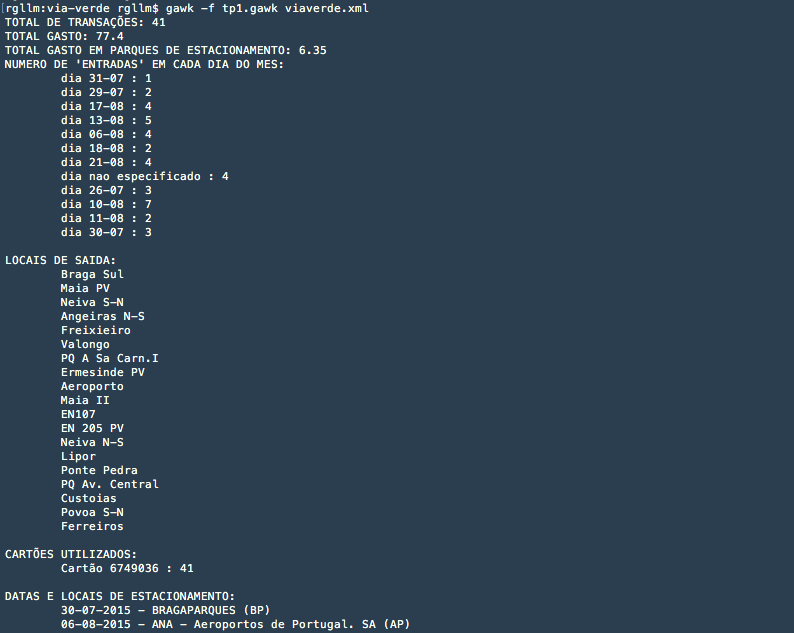
\includegraphics[scale=0.5]{1}
\end{center}
\\
Ao analisar um ficheiro XML com a estrutura da via verde são obtidos alguns dados interessantes para o utilizador recorrendo ao programa desenvolvido. O programa calcula o número total de transações, o total gasto e o total gasto só em parques de estacionamento, para além de indicar o número de entradas em cada mês, os locais de saída, os cartões utilizados e as datas e os locais de estacionamento.
\\
\\
\textbf{\underline{Álbum Fotográfico em HTML}}
\\
\\
\begin{center}
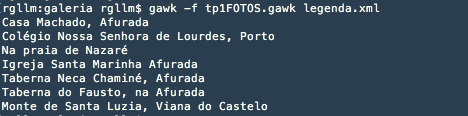
\includegraphics[scale=1]{2}
\end{center}
\\
\\
\begin{center}
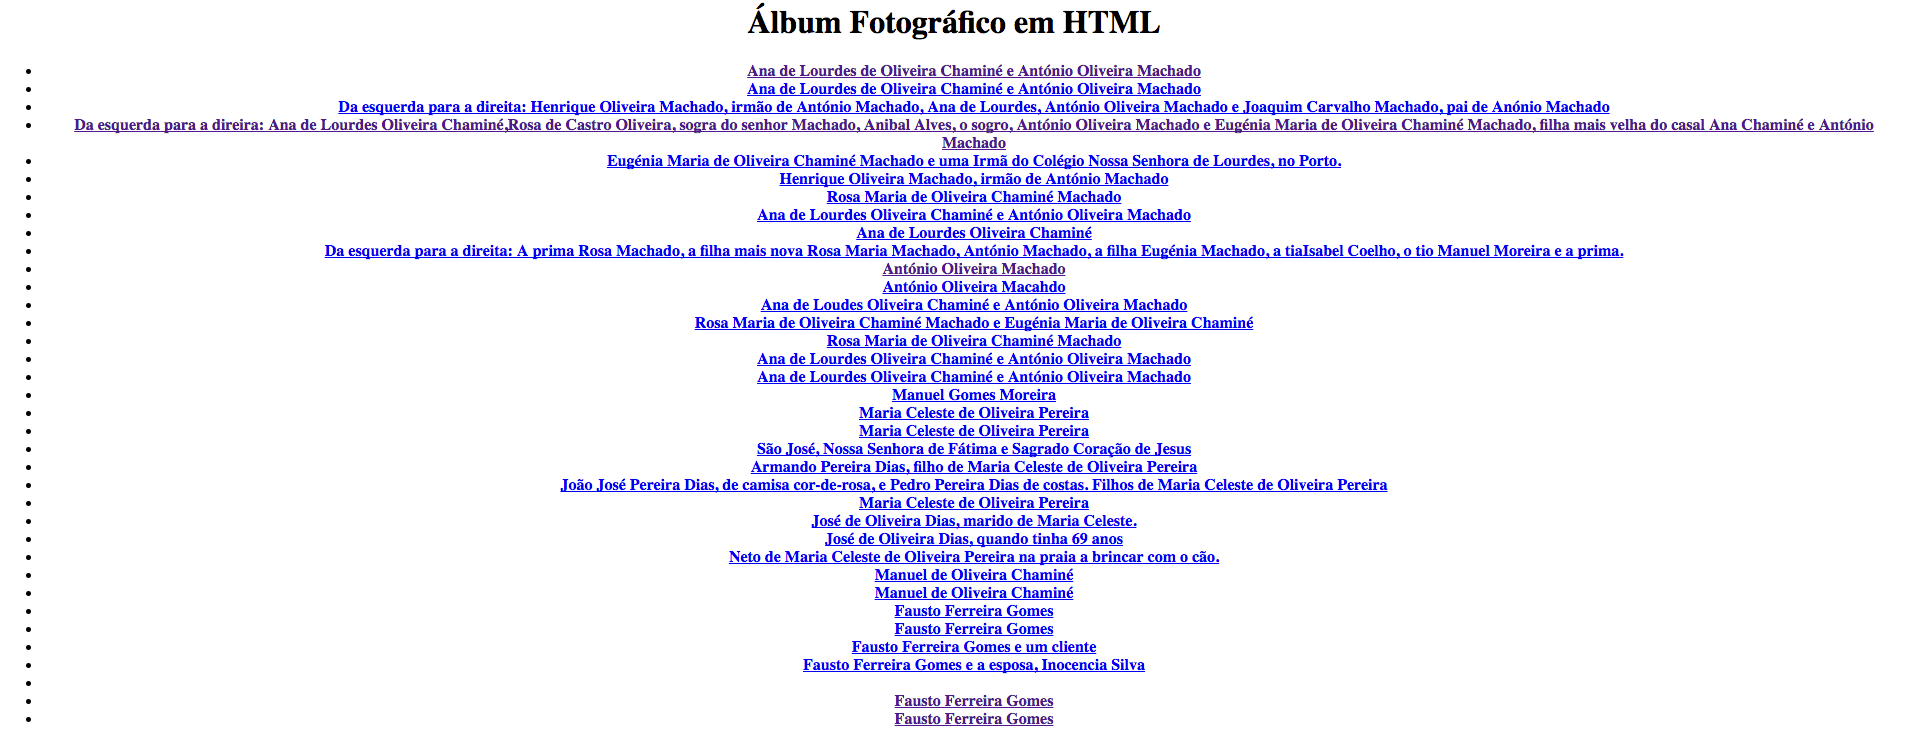
\includegraphics[scale=0.2]{3}
\end{center}
\\
\\
\begin{center}
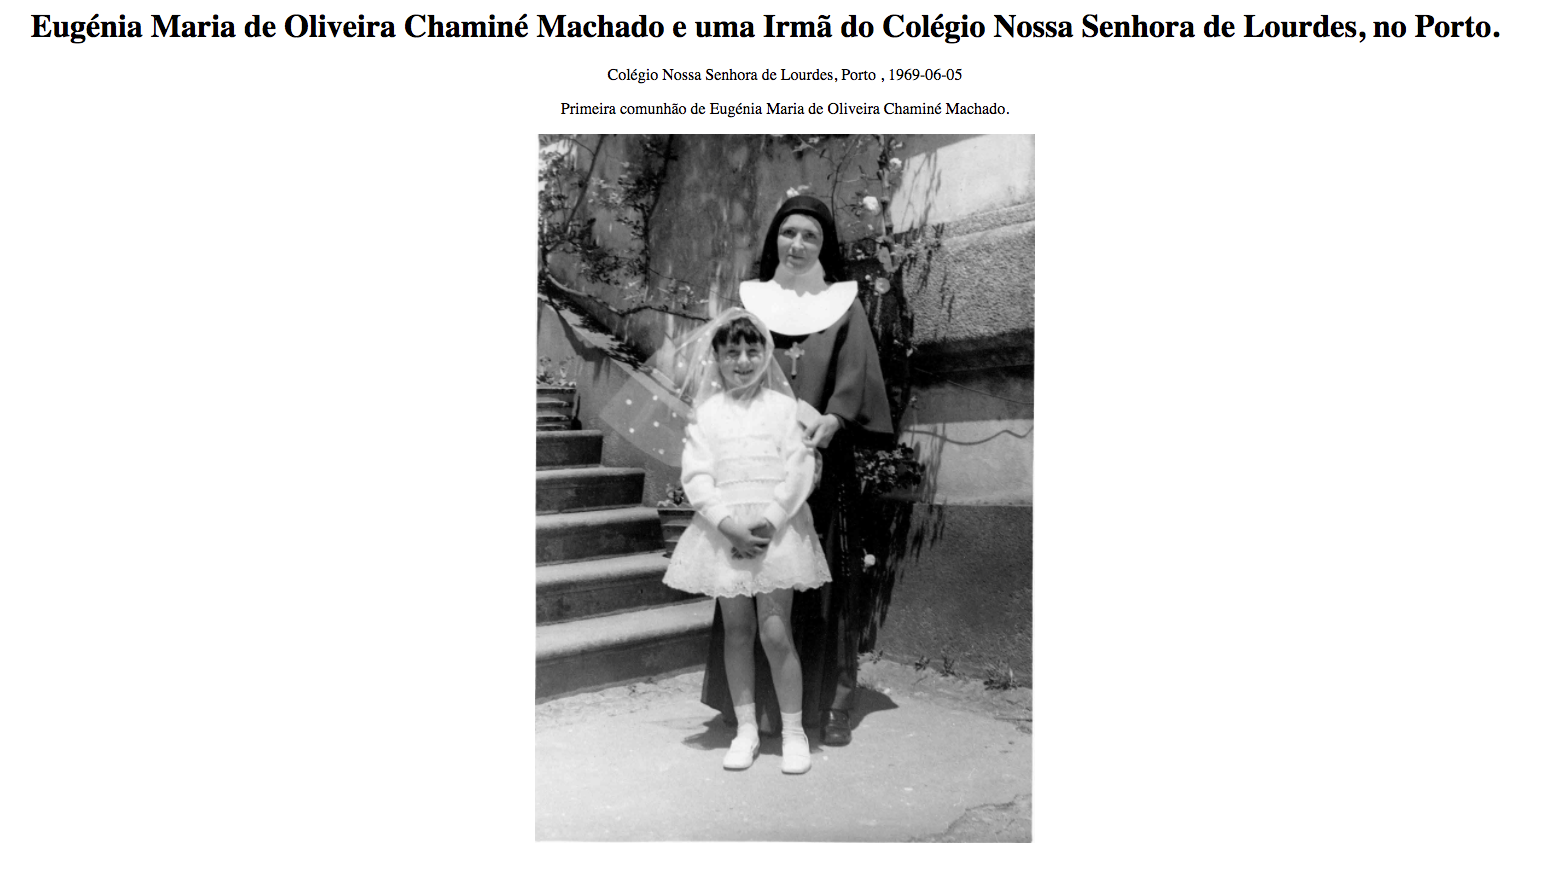
\includegraphics[scale=0.3]{4}
\end{center}
\newpage
\begin{center}
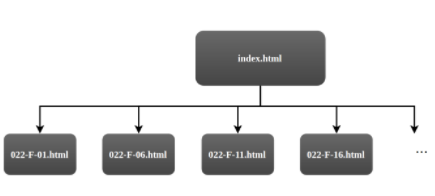
\includegraphics[scale=1]{5}
\end{center}
\\
\\
Quando o programa é executado, os resultados são apresentados de duas maneiras distintas:
\\
\begin{itemize}
    \item No terminal/bash são listados todos os locais fotografados, sem repetições;
    \item Por outro lado são também gerados os ficheiros index.html e um ficheiro nome-da-foto.html para cada uma das fotos. O ficheiro index.html apresenta uma lista das fotos disponíveis com o respetivo apontador para o ficheiro da foto, onde são mostrados todos os dados relativo aquela foto.
\end{itemize}
\\
\\
\chapter{Conclusão} \label{concl}
Durante todo o desenvolvimento dos dois programas, tentámos que o código se aplicasse a qualquer ficheiro com o mesmo formato e fosse o mais compacto possível. Contudo, os programas desenvolvidos não cobrem algumas exceções e por se tratar de um trabalho académico não têm algumas verificações que porventura num programa em produção seriam necessárias.
No geral, os objetivos esperados para o programa foram alcançados e obtemos uma solução sólida para o problema apresentado. Destacamos ainda alguns pontos:
\\
\begin{itemize}
    \item No trabalho do álbum em HTML foi gerado um ficheiro para cada foto e um ficheiro central com apontadores para estes em alternativa a haver apenas um ficheiro com toda a informação das fotos.
    \item No trabalho da via verde foram filtrados mais dados do que aqueles inicialmente previstos no guião. Dos quais destacamos: listagem das datas e locais de estacionamento, os cartões utilizados e o total de transações.
    \item Destacamos também que funções auxiliares para cada um dos projetos são codificadas em ficheiros aparte (ficheiro gets.gawk e ficheiro funcs.gawk) para garantir a uniformização do código.
\end{itemize}
\\
Como trabalho futuro sugerimos:
\\
\begin{itemize}
    \item Mais verificações para garantir que não ocorrem erros de leitura;
    \item Tratamento das legendas das fotos com o parâmetro “alt”.
    \item Navegação entre fotografias.
\end{itemize}

\appendix
\chapter{Código GAWK}

Lista-se a seguir o código desenvolvido.
\\
\textbf{\underline{Processador de transações da Via Verde}}

\underline{Ficheiro gets.gawk}

\lstinputlisting{gets.gawk}
\newpage
\underline{Ficheiro tp1.gawk}

\lstinputlisting{tp1.gawk}
\newpage
\textbf{\underline{Álbum Fotográfico em HTML}}

\underline{Ficheiro funcs.gawk}

\lstinputlisting{funcs.gawk}
\newpage
\underline{Ficheiro tp1FOTOS.gawk}

\lstinputlisting{tp1FOTOS.gawk}

\bibliographystyle{alpha}
\bibliography{relprojLayout}







\end{document}
